% Options for packages loaded elsewhere
\PassOptionsToPackage{unicode}{hyperref}
\PassOptionsToPackage{hyphens}{url}
\PassOptionsToPackage{dvipsnames,svgnames,x11names}{xcolor}
%
\documentclass[
  letterpaper,
  DIV=11,
  numbers=noendperiod]{scrreprt}

\usepackage{amsmath,amssymb}
\usepackage{iftex}
\ifPDFTeX
  \usepackage[T1]{fontenc}
  \usepackage[utf8]{inputenc}
  \usepackage{textcomp} % provide euro and other symbols
\else % if luatex or xetex
  \usepackage{unicode-math}
  \defaultfontfeatures{Scale=MatchLowercase}
  \defaultfontfeatures[\rmfamily]{Ligatures=TeX,Scale=1}
\fi
\usepackage{lmodern}
\ifPDFTeX\else  
    % xetex/luatex font selection
\fi
% Use upquote if available, for straight quotes in verbatim environments
\IfFileExists{upquote.sty}{\usepackage{upquote}}{}
\IfFileExists{microtype.sty}{% use microtype if available
  \usepackage[]{microtype}
  \UseMicrotypeSet[protrusion]{basicmath} % disable protrusion for tt fonts
}{}
\makeatletter
\@ifundefined{KOMAClassName}{% if non-KOMA class
  \IfFileExists{parskip.sty}{%
    \usepackage{parskip}
  }{% else
    \setlength{\parindent}{0pt}
    \setlength{\parskip}{6pt plus 2pt minus 1pt}}
}{% if KOMA class
  \KOMAoptions{parskip=half}}
\makeatother
\usepackage{xcolor}
\setlength{\emergencystretch}{3em} % prevent overfull lines
\setcounter{secnumdepth}{5}
% Make \paragraph and \subparagraph free-standing
\ifx\paragraph\undefined\else
  \let\oldparagraph\paragraph
  \renewcommand{\paragraph}[1]{\oldparagraph{#1}\mbox{}}
\fi
\ifx\subparagraph\undefined\else
  \let\oldsubparagraph\subparagraph
  \renewcommand{\subparagraph}[1]{\oldsubparagraph{#1}\mbox{}}
\fi

\usepackage{color}
\usepackage{fancyvrb}
\newcommand{\VerbBar}{|}
\newcommand{\VERB}{\Verb[commandchars=\\\{\}]}
\DefineVerbatimEnvironment{Highlighting}{Verbatim}{commandchars=\\\{\}}
% Add ',fontsize=\small' for more characters per line
\usepackage{framed}
\definecolor{shadecolor}{RGB}{241,243,245}
\newenvironment{Shaded}{\begin{snugshade}}{\end{snugshade}}
\newcommand{\AlertTok}[1]{\textcolor[rgb]{0.68,0.00,0.00}{#1}}
\newcommand{\AnnotationTok}[1]{\textcolor[rgb]{0.37,0.37,0.37}{#1}}
\newcommand{\AttributeTok}[1]{\textcolor[rgb]{0.40,0.45,0.13}{#1}}
\newcommand{\BaseNTok}[1]{\textcolor[rgb]{0.68,0.00,0.00}{#1}}
\newcommand{\BuiltInTok}[1]{\textcolor[rgb]{0.00,0.23,0.31}{#1}}
\newcommand{\CharTok}[1]{\textcolor[rgb]{0.13,0.47,0.30}{#1}}
\newcommand{\CommentTok}[1]{\textcolor[rgb]{0.37,0.37,0.37}{#1}}
\newcommand{\CommentVarTok}[1]{\textcolor[rgb]{0.37,0.37,0.37}{\textit{#1}}}
\newcommand{\ConstantTok}[1]{\textcolor[rgb]{0.56,0.35,0.01}{#1}}
\newcommand{\ControlFlowTok}[1]{\textcolor[rgb]{0.00,0.23,0.31}{#1}}
\newcommand{\DataTypeTok}[1]{\textcolor[rgb]{0.68,0.00,0.00}{#1}}
\newcommand{\DecValTok}[1]{\textcolor[rgb]{0.68,0.00,0.00}{#1}}
\newcommand{\DocumentationTok}[1]{\textcolor[rgb]{0.37,0.37,0.37}{\textit{#1}}}
\newcommand{\ErrorTok}[1]{\textcolor[rgb]{0.68,0.00,0.00}{#1}}
\newcommand{\ExtensionTok}[1]{\textcolor[rgb]{0.00,0.23,0.31}{#1}}
\newcommand{\FloatTok}[1]{\textcolor[rgb]{0.68,0.00,0.00}{#1}}
\newcommand{\FunctionTok}[1]{\textcolor[rgb]{0.28,0.35,0.67}{#1}}
\newcommand{\ImportTok}[1]{\textcolor[rgb]{0.00,0.46,0.62}{#1}}
\newcommand{\InformationTok}[1]{\textcolor[rgb]{0.37,0.37,0.37}{#1}}
\newcommand{\KeywordTok}[1]{\textcolor[rgb]{0.00,0.23,0.31}{#1}}
\newcommand{\NormalTok}[1]{\textcolor[rgb]{0.00,0.23,0.31}{#1}}
\newcommand{\OperatorTok}[1]{\textcolor[rgb]{0.37,0.37,0.37}{#1}}
\newcommand{\OtherTok}[1]{\textcolor[rgb]{0.00,0.23,0.31}{#1}}
\newcommand{\PreprocessorTok}[1]{\textcolor[rgb]{0.68,0.00,0.00}{#1}}
\newcommand{\RegionMarkerTok}[1]{\textcolor[rgb]{0.00,0.23,0.31}{#1}}
\newcommand{\SpecialCharTok}[1]{\textcolor[rgb]{0.37,0.37,0.37}{#1}}
\newcommand{\SpecialStringTok}[1]{\textcolor[rgb]{0.13,0.47,0.30}{#1}}
\newcommand{\StringTok}[1]{\textcolor[rgb]{0.13,0.47,0.30}{#1}}
\newcommand{\VariableTok}[1]{\textcolor[rgb]{0.07,0.07,0.07}{#1}}
\newcommand{\VerbatimStringTok}[1]{\textcolor[rgb]{0.13,0.47,0.30}{#1}}
\newcommand{\WarningTok}[1]{\textcolor[rgb]{0.37,0.37,0.37}{\textit{#1}}}

\providecommand{\tightlist}{%
  \setlength{\itemsep}{0pt}\setlength{\parskip}{0pt}}\usepackage{longtable,booktabs,array}
\usepackage{calc} % for calculating minipage widths
% Correct order of tables after \paragraph or \subparagraph
\usepackage{etoolbox}
\makeatletter
\patchcmd\longtable{\par}{\if@noskipsec\mbox{}\fi\par}{}{}
\makeatother
% Allow footnotes in longtable head/foot
\IfFileExists{footnotehyper.sty}{\usepackage{footnotehyper}}{\usepackage{footnote}}
\makesavenoteenv{longtable}
\usepackage{graphicx}
\makeatletter
\def\maxwidth{\ifdim\Gin@nat@width>\linewidth\linewidth\else\Gin@nat@width\fi}
\def\maxheight{\ifdim\Gin@nat@height>\textheight\textheight\else\Gin@nat@height\fi}
\makeatother
% Scale images if necessary, so that they will not overflow the page
% margins by default, and it is still possible to overwrite the defaults
% using explicit options in \includegraphics[width, height, ...]{}
\setkeys{Gin}{width=\maxwidth,height=\maxheight,keepaspectratio}
% Set default figure placement to htbp
\makeatletter
\def\fps@figure{htbp}
\makeatother

\KOMAoption{captions}{tableheading}
\makeatletter
\@ifpackageloaded{tcolorbox}{}{\usepackage[skins,breakable]{tcolorbox}}
\@ifpackageloaded{fontawesome5}{}{\usepackage{fontawesome5}}
\definecolor{quarto-callout-color}{HTML}{909090}
\definecolor{quarto-callout-note-color}{HTML}{0758E5}
\definecolor{quarto-callout-important-color}{HTML}{CC1914}
\definecolor{quarto-callout-warning-color}{HTML}{EB9113}
\definecolor{quarto-callout-tip-color}{HTML}{00A047}
\definecolor{quarto-callout-caution-color}{HTML}{FC5300}
\definecolor{quarto-callout-color-frame}{HTML}{acacac}
\definecolor{quarto-callout-note-color-frame}{HTML}{4582ec}
\definecolor{quarto-callout-important-color-frame}{HTML}{d9534f}
\definecolor{quarto-callout-warning-color-frame}{HTML}{f0ad4e}
\definecolor{quarto-callout-tip-color-frame}{HTML}{02b875}
\definecolor{quarto-callout-caution-color-frame}{HTML}{fd7e14}
\makeatother
\makeatletter
\@ifpackageloaded{bookmark}{}{\usepackage{bookmark}}
\makeatother
\makeatletter
\@ifpackageloaded{caption}{}{\usepackage{caption}}
\AtBeginDocument{%
\ifdefined\contentsname
  \renewcommand*\contentsname{Table of contents}
\else
  \newcommand\contentsname{Table of contents}
\fi
\ifdefined\listfigurename
  \renewcommand*\listfigurename{List of Figures}
\else
  \newcommand\listfigurename{List of Figures}
\fi
\ifdefined\listtablename
  \renewcommand*\listtablename{List of Tables}
\else
  \newcommand\listtablename{List of Tables}
\fi
\ifdefined\figurename
  \renewcommand*\figurename{Figure}
\else
  \newcommand\figurename{Figure}
\fi
\ifdefined\tablename
  \renewcommand*\tablename{Table}
\else
  \newcommand\tablename{Table}
\fi
}
\@ifpackageloaded{float}{}{\usepackage{float}}
\floatstyle{ruled}
\@ifundefined{c@chapter}{\newfloat{codelisting}{h}{lop}}{\newfloat{codelisting}{h}{lop}[chapter]}
\floatname{codelisting}{Listing}
\newcommand*\listoflistings{\listof{codelisting}{List of Listings}}
\makeatother
\makeatletter
\makeatother
\makeatletter
\@ifpackageloaded{caption}{}{\usepackage{caption}}
\@ifpackageloaded{subcaption}{}{\usepackage{subcaption}}
\makeatother
\ifLuaTeX
  \usepackage{selnolig}  % disable illegal ligatures
\fi
\usepackage{bookmark}

\IfFileExists{xurl.sty}{\usepackage{xurl}}{} % add URL line breaks if available
\urlstyle{same} % disable monospaced font for URLs
\hypersetup{
  pdftitle={Estatistica Educacional},
  pdfauthor={Elton Pereira dos Santos},
  colorlinks=true,
  linkcolor={blue},
  filecolor={Maroon},
  citecolor={Blue},
  urlcolor={Blue},
  pdfcreator={LaTeX via pandoc}}

\title{Estatistica Educacional}
\usepackage{etoolbox}
\makeatletter
\providecommand{\subtitle}[1]{% add subtitle to \maketitle
  \apptocmd{\@title}{\par {\large #1 \par}}{}{}
}
\makeatother
\subtitle{Disciplina de Estatistica}
\author{Elton Pereira dos Santos}
\date{2024-06-12}

\begin{document}
\maketitle

\renewcommand*\contentsname{Table of contents}
{
\hypersetup{linkcolor=}
\setcounter{tocdepth}{2}
\tableofcontents
}
\bookmarksetup{startatroot}

\chapter*{Preface}\label{preface}
\addcontentsline{toc}{chapter}{Preface}

\markboth{Preface}{Preface}

Edumetria no Quarto book.

É o método de mensuração das variáveis relacionadas ao processo de
ensino e aprendizagem conjugado com interpretações qualitativas,
sensíveis e sociais. É a interface entre a análise quantitativa e
qualitativa na área do conhecimento da Educação que emerge uma
síntese.{[}1{]}{[}2{]} É a aplicação da Estatística à área de Educação,
com forte colaboração da Pedagogia. Essa Estatística Educacional é
composta por muitos métodos, destacando-se a Teoria Clássica de Medidas,
a Teoria da Resposta ao Item, Modelagem Linear Hierarquica, Regressão
Quantílica, dentre outras (Andrade, Tavares, Valle, 2000).

To learn more about Quarto books visit
\url{https://quarto.org/docs/books}.

\bookmarksetup{startatroot}

\chapter{Introduction}\label{introduction}

\section{Funções e Distribruiçoes
Graficas}\label{funuxe7uxf5es-e-distribruiuxe7oes-graficas}

\begin{tcolorbox}[enhanced jigsaw, toptitle=1mm, rightrule=.15mm, title=\textcolor{quarto-callout-note-color}{\faInfo}\hspace{0.5em}{Note}, colframe=quarto-callout-note-color-frame, colback=white, colbacktitle=quarto-callout-note-color!10!white, leftrule=.75mm, opacityback=0, breakable, coltitle=black, opacitybacktitle=0.6, bottomtitle=1mm, titlerule=0mm, arc=.35mm, bottomrule=.15mm, toprule=.15mm, left=2mm]

Para gerar o gráfico das funções
\[f(x)=x2−5x+6 \\ f(x) = x^2 - 5x + 6 \\  f(x)=x2−5x+6\] no intervalo.

\(x∈[0,4]sin[0, 4]x∈[0,4]\) utilizando a linguagem de programação R,
você pode seguir os seguintes passos:

\end{tcolorbox}

\subsection{Gráfico da função f(x) = x\^{}2 - 5x +
6}\label{gruxe1fico-da-funuxe7uxe3o-fx-x2---5x-6}

\begin{Shaded}
\begin{Highlighting}[]
\CommentTok{\# Definir a função}
\NormalTok{f }\OtherTok{\textless{}{-}} \ControlFlowTok{function}\NormalTok{(x) \{}
  \FunctionTok{return}\NormalTok{(x}\SpecialCharTok{\^{}}\DecValTok{2} \SpecialCharTok{{-}} \DecValTok{5}\SpecialCharTok{*}\NormalTok{x }\SpecialCharTok{+} \DecValTok{6}\NormalTok{)}
\NormalTok{\}}

\CommentTok{\# Gerar os valores de x no intervalo [0, 4]}
\NormalTok{x\_vals }\OtherTok{\textless{}{-}} \FunctionTok{seq}\NormalTok{(}\DecValTok{0}\NormalTok{, }\DecValTok{4}\NormalTok{, }\AttributeTok{by =} \FloatTok{0.01}\NormalTok{)}

\CommentTok{\# Calcular os valores de f(x) para cada valor de x}
\NormalTok{y\_vals }\OtherTok{\textless{}{-}} \FunctionTok{f}\NormalTok{(x\_vals)}

\CommentTok{\# Plotar o gráfico}
\FunctionTok{plot}\NormalTok{(x\_vals, y\_vals, }\AttributeTok{type =} \StringTok{"l"}\NormalTok{, }\AttributeTok{col =} \StringTok{"blue"}\NormalTok{, }\AttributeTok{lwd =} \DecValTok{2}\NormalTok{,}
     \AttributeTok{xlab =} \StringTok{"x"}\NormalTok{, }\AttributeTok{ylab =} \StringTok{"f(x)"}\NormalTok{, }\AttributeTok{main =} \StringTok{"Gráfico da função f(x) = x\^{}2 {-} 5x + 6"}\NormalTok{)}
\end{Highlighting}
\end{Shaded}

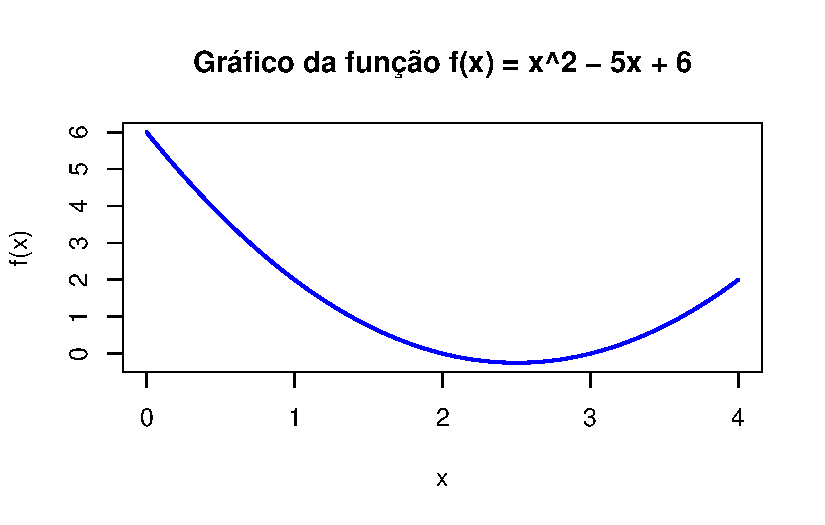
\includegraphics{intro_files/figure-pdf/unnamed-chunk-1-1.pdf}

\subsection{Função de densidade e Distribuição da
N(0,1).}\label{funuxe7uxe3o-de-densidade-e-distribuiuxe7uxe3o-da-n01.}

Que na pratica seria a distribuição normal (0,1), em um lado a densidade
em que ela assume e no outro a distribuição.

\begin{Shaded}
\begin{Highlighting}[]
\CommentTok{\# Gerar os valores de x para o gráfico}
\NormalTok{x\_vals }\OtherTok{\textless{}{-}} \FunctionTok{seq}\NormalTok{(}\SpecialCharTok{{-}}\DecValTok{4}\NormalTok{, }\DecValTok{4}\NormalTok{, }\AttributeTok{by =} \FloatTok{0.01}\NormalTok{)}

\CommentTok{\# Calcular a densidade da N(0,1) (função de densidade)}
\NormalTok{density\_vals }\OtherTok{\textless{}{-}} \FunctionTok{dnorm}\NormalTok{(x\_vals, }\AttributeTok{mean =} \DecValTok{0}\NormalTok{, }\AttributeTok{sd =} \DecValTok{1}\NormalTok{)}

\CommentTok{\# Calcular a função de distribuição acumulada (CDF) da N(0,1)}
\NormalTok{cdf\_vals }\OtherTok{\textless{}{-}} \FunctionTok{pnorm}\NormalTok{(x\_vals, }\AttributeTok{mean =} \DecValTok{0}\NormalTok{, }\AttributeTok{sd =} \DecValTok{1}\NormalTok{)}

\CommentTok{\# Plotar ambos os gráficos em um só}
\FunctionTok{par}\NormalTok{(}\AttributeTok{mfrow =} \FunctionTok{c}\NormalTok{(}\DecValTok{1}\NormalTok{, }\DecValTok{2}\NormalTok{))  }\CommentTok{\# Dividir a tela em 2 gráficos (1 linha, 2 colunas)}

\CommentTok{\# Gráfico da densidade}
\FunctionTok{plot}\NormalTok{(x\_vals, density\_vals, }\AttributeTok{type =} \StringTok{"l"}\NormalTok{, }\AttributeTok{col =} \StringTok{"blue"}\NormalTok{, }\AttributeTok{lwd =} \DecValTok{2}\NormalTok{,}
     \AttributeTok{xlab =} \StringTok{"x"}\NormalTok{, }\AttributeTok{ylab =} \StringTok{"Densidade"}\NormalTok{, }\AttributeTok{main =} \StringTok{"Densidade da N(0,1)"}\NormalTok{)}

\CommentTok{\# Gráfico da função de distribuição acumulada (CDF)}
\FunctionTok{plot}\NormalTok{(x\_vals, cdf\_vals, }\AttributeTok{type =} \StringTok{"l"}\NormalTok{, }\AttributeTok{col =} \StringTok{"red"}\NormalTok{, }\AttributeTok{lwd =} \DecValTok{2}\NormalTok{,}
     \AttributeTok{xlab =} \StringTok{"x"}\NormalTok{, }\AttributeTok{ylab =} \StringTok{"F(x)"}\NormalTok{, }\AttributeTok{main =} \StringTok{"Função de Distribuição da N(0,1)"}\NormalTok{)}
\end{Highlighting}
\end{Shaded}

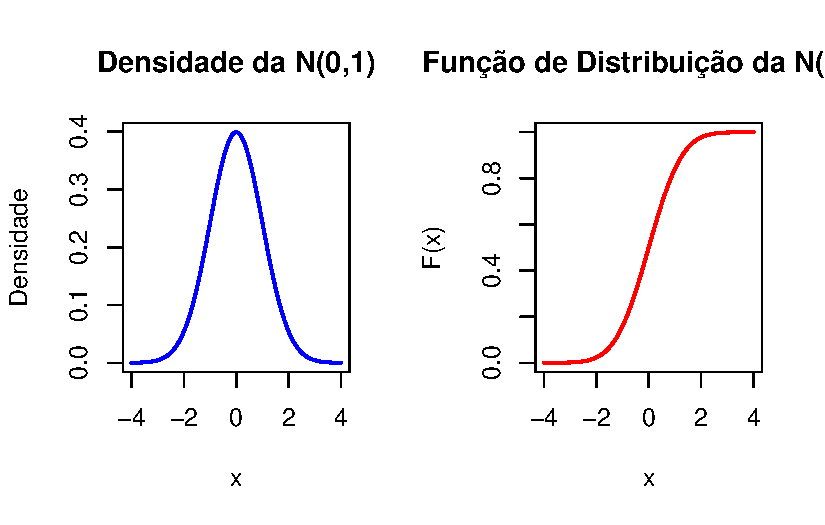
\includegraphics{intro_files/figure-pdf/unnamed-chunk-2-1.pdf}

\begin{Shaded}
\begin{Highlighting}[]
\CommentTok{\# Restaurar o layout do gráfico}
\FunctionTok{par}\NormalTok{(}\AttributeTok{mfrow =} \FunctionTok{c}\NormalTok{(}\DecValTok{1}\NormalTok{, }\DecValTok{1}\NormalTok{))  }\CommentTok{\# Voltar para o layout padrão}
\end{Highlighting}
\end{Shaded}

\begin{Shaded}
\begin{Highlighting}[]
 \CommentTok{\#Definir a função f(x)}
\NormalTok{f }\OtherTok{\textless{}{-}} \ControlFlowTok{function}\NormalTok{(x, a, b, D) \{}
  \FunctionTok{return}\NormalTok{(}\DecValTok{1} \SpecialCharTok{/}\NormalTok{ (}\DecValTok{1} \SpecialCharTok{+} \FunctionTok{exp}\NormalTok{(}\SpecialCharTok{{-}}\NormalTok{D }\SpecialCharTok{*}\NormalTok{ a }\SpecialCharTok{*}\NormalTok{ (x }\SpecialCharTok{{-}}\NormalTok{ b))))}
\NormalTok{\}}

\CommentTok{\# Definir os parâmetros}
\NormalTok{a }\OtherTok{\textless{}{-}} \FloatTok{1.5}
\NormalTok{b }\OtherTok{\textless{}{-}} \DecValTok{1}
\NormalTok{D1 }\OtherTok{\textless{}{-}} \DecValTok{1}
\NormalTok{D2 }\OtherTok{\textless{}{-}} \FloatTok{1.7}

\CommentTok{\# Gerar os valores de x no intervalo}
\NormalTok{x\_vals }\OtherTok{\textless{}{-}} \FunctionTok{seq}\NormalTok{(}\SpecialCharTok{{-}}\DecValTok{5}\NormalTok{, }\DecValTok{5}\NormalTok{, }\AttributeTok{by =} \FloatTok{0.01}\NormalTok{)}

\CommentTok{\# Calcular os valores de f(x) para os dois casos de D}
\NormalTok{y\_vals\_D1 }\OtherTok{\textless{}{-}} \FunctionTok{f}\NormalTok{(x\_vals, a, b, D1)}
\NormalTok{y\_vals\_D2 }\OtherTok{\textless{}{-}} \FunctionTok{f}\NormalTok{(x\_vals, a, b, D2)}

\CommentTok{\# Plotar os gráficos}
\FunctionTok{plot}\NormalTok{(x\_vals, y\_vals\_D1, }\AttributeTok{type =} \StringTok{"l"}\NormalTok{, }\AttributeTok{col =} \StringTok{"blue"}\NormalTok{, }\AttributeTok{lwd =} \DecValTok{2}\NormalTok{, }
     \AttributeTok{xlab =} \StringTok{"x"}\NormalTok{, }\AttributeTok{ylab =} \StringTok{"f(x)"}\NormalTok{, }\AttributeTok{main =} \StringTok{"Gráfico de f(x) para D=1 e D=1.7"}\NormalTok{)}
\FunctionTok{lines}\NormalTok{(x\_vals, y\_vals\_D2, }\AttributeTok{col =} \StringTok{"red"}\NormalTok{, }\AttributeTok{lwd =} \DecValTok{2}\NormalTok{)}

\CommentTok{\# Adicionar uma legenda}
\FunctionTok{legend}\NormalTok{(}\StringTok{"topleft"}\NormalTok{, }\AttributeTok{legend =} \FunctionTok{c}\NormalTok{(}\StringTok{"D = 1"}\NormalTok{, }\StringTok{"D = 1.7"}\NormalTok{), }\AttributeTok{col =} \FunctionTok{c}\NormalTok{(}\StringTok{"blue"}\NormalTok{, }\StringTok{"red"}\NormalTok{), }\AttributeTok{lwd =} \DecValTok{2}\NormalTok{)}
\end{Highlighting}
\end{Shaded}

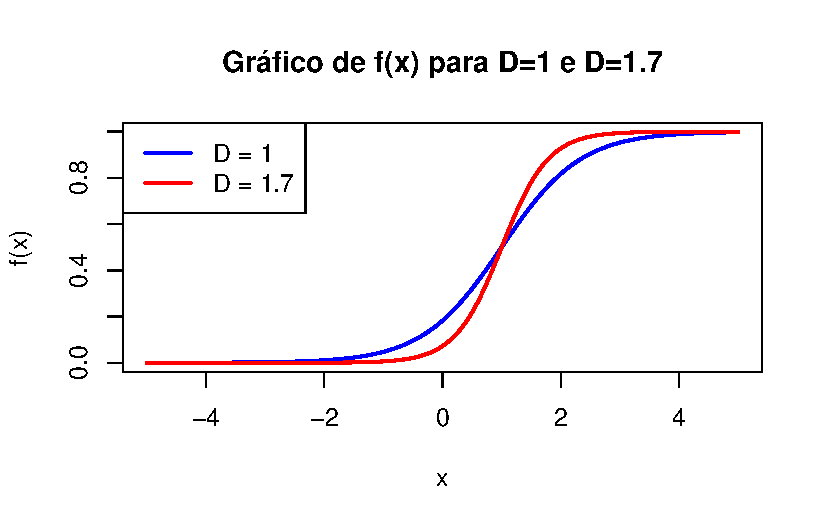
\includegraphics{intro_files/figure-pdf/unnamed-chunk-3-1.pdf}

\begin{Shaded}
\begin{Highlighting}[]
\CommentTok{\# Definir a função f(x)}
\NormalTok{f }\OtherTok{\textless{}{-}} \ControlFlowTok{function}\NormalTok{(x, a, b, D) \{}
  \FunctionTok{return}\NormalTok{(}\DecValTok{1} \SpecialCharTok{/}\NormalTok{ (}\DecValTok{1} \SpecialCharTok{+} \FunctionTok{exp}\NormalTok{(}\SpecialCharTok{{-}}\NormalTok{D }\SpecialCharTok{*}\NormalTok{ a }\SpecialCharTok{*}\NormalTok{ (x }\SpecialCharTok{{-}}\NormalTok{ b))))}
\NormalTok{\}}

\CommentTok{\# Definir os parâmetros}
\NormalTok{a }\OtherTok{\textless{}{-}} \FloatTok{1.5}
\NormalTok{b }\OtherTok{\textless{}{-}} \DecValTok{1}
\NormalTok{D1 }\OtherTok{\textless{}{-}} \DecValTok{1}
\NormalTok{D2 }\OtherTok{\textless{}{-}} \FloatTok{1.7}

\CommentTok{\# Gerar os valores de x no intervalo}
\NormalTok{x\_vals }\OtherTok{\textless{}{-}} \FunctionTok{seq}\NormalTok{(}\SpecialCharTok{{-}}\DecValTok{5}\NormalTok{, }\DecValTok{5}\NormalTok{, }\AttributeTok{by =} \FloatTok{0.01}\NormalTok{)}

\CommentTok{\# Calcular os valores de f(x) para os dois casos de D}
\NormalTok{y\_vals\_D1 }\OtherTok{\textless{}{-}} \FunctionTok{f}\NormalTok{(x\_vals, a, b, D1)}
\NormalTok{y\_vals\_D2 }\OtherTok{\textless{}{-}} \FunctionTok{f}\NormalTok{(x\_vals, a, b, D2)}

\CommentTok{\# Plotar os gráficos}
\FunctionTok{plot}\NormalTok{(x\_vals, y\_vals\_D1, }\AttributeTok{type =} \StringTok{"l"}\NormalTok{, }\AttributeTok{col =} \StringTok{"blue"}\NormalTok{, }\AttributeTok{lwd =} \DecValTok{2}\NormalTok{, }
     \AttributeTok{xlab =} \StringTok{"x"}\NormalTok{, }\AttributeTok{ylab =} \StringTok{"f(x)"}\NormalTok{, }\AttributeTok{main =} \StringTok{"Gráfico de f(x) para D=1 e D=1.7"}\NormalTok{)}
\FunctionTok{lines}\NormalTok{(x\_vals, y\_vals\_D2, }\AttributeTok{col =} \StringTok{"red"}\NormalTok{, }\AttributeTok{lwd =} \DecValTok{2}\NormalTok{)}

\CommentTok{\# Adicionar uma legenda}
\FunctionTok{legend}\NormalTok{(}\StringTok{"topleft"}\NormalTok{, }\AttributeTok{legend =} \FunctionTok{c}\NormalTok{(}\StringTok{"D = 1"}\NormalTok{, }\StringTok{"D = 1.7"}\NormalTok{), }\AttributeTok{col =} \FunctionTok{c}\NormalTok{(}\StringTok{"blue"}\NormalTok{, }\StringTok{"red"}\NormalTok{), }\AttributeTok{lwd =} \DecValTok{2}\NormalTok{)}
\end{Highlighting}
\end{Shaded}

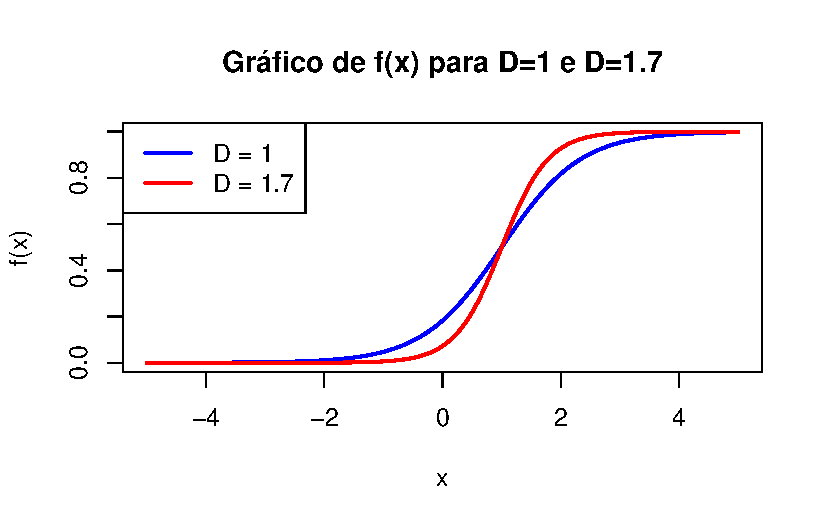
\includegraphics{intro_files/figure-pdf/unnamed-chunk-4-1.pdf}

\begin{Shaded}
\begin{Highlighting}[]
\CommentTok{\# Definir a função f(x)}
\NormalTok{f }\OtherTok{\textless{}{-}} \ControlFlowTok{function}\NormalTok{(x, a, b, c, D) \{}
  \FunctionTok{return}\NormalTok{(c }\SpecialCharTok{+}\NormalTok{ (}\DecValTok{1} \SpecialCharTok{{-}}\NormalTok{ c) }\SpecialCharTok{/}\NormalTok{ (}\DecValTok{1} \SpecialCharTok{+} \FunctionTok{exp}\NormalTok{(}\SpecialCharTok{{-}}\NormalTok{D }\SpecialCharTok{*}\NormalTok{ a }\SpecialCharTok{*}\NormalTok{ (x }\SpecialCharTok{{-}}\NormalTok{ b))))}
\NormalTok{\}}

\CommentTok{\# Definir os parâmetros}
\NormalTok{a }\OtherTok{\textless{}{-}} \FloatTok{1.5}
\NormalTok{b }\OtherTok{\textless{}{-}} \DecValTok{1}
\NormalTok{c }\OtherTok{\textless{}{-}} \FloatTok{0.2}
\NormalTok{D }\OtherTok{\textless{}{-}} \FloatTok{1.7}

\CommentTok{\# Gerar os valores de x no intervalo}
\NormalTok{x\_vals }\OtherTok{\textless{}{-}} \FunctionTok{seq}\NormalTok{(}\SpecialCharTok{{-}}\DecValTok{5}\NormalTok{, }\DecValTok{5}\NormalTok{, }\AttributeTok{by =} \FloatTok{0.01}\NormalTok{)}

\CommentTok{\# Calcular os valores de f(x) para cada valor de x}
\NormalTok{y\_vals }\OtherTok{\textless{}{-}} \FunctionTok{f}\NormalTok{(x\_vals, a, b, c, D)}

\CommentTok{\# Plotar o gráfico}
\FunctionTok{plot}\NormalTok{(x\_vals, y\_vals, }\AttributeTok{type =} \StringTok{"l"}\NormalTok{, }\AttributeTok{col =} \StringTok{"blue"}\NormalTok{, }\AttributeTok{lwd =} \DecValTok{2}\NormalTok{,}
     \AttributeTok{xlab =} \StringTok{"x"}\NormalTok{, }\AttributeTok{ylab =} \StringTok{"f(x)"}\NormalTok{, }\AttributeTok{main =} \StringTok{"Gráfico da função f(x) = c + (1 {-} c) / (1 + exp({-}D a (x {-} b)))"}\NormalTok{)}
\end{Highlighting}
\end{Shaded}

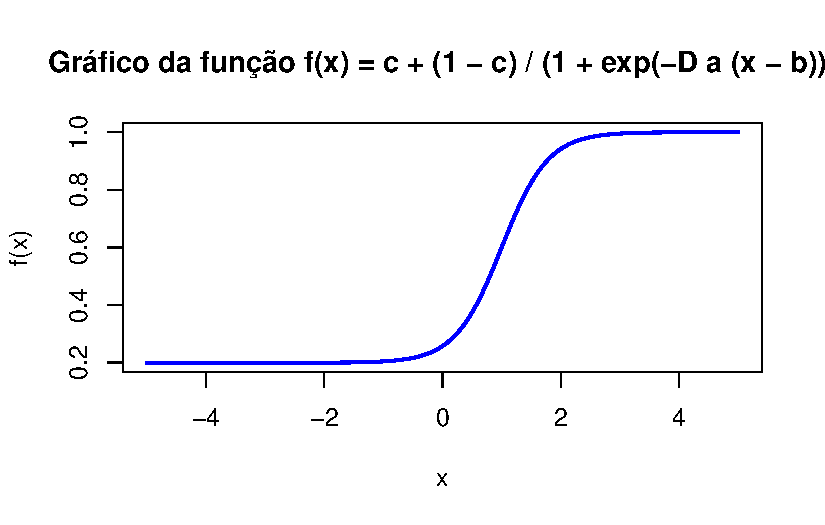
\includegraphics{intro_files/figure-pdf/unnamed-chunk-5-1.pdf}

\begin{Shaded}
\begin{Highlighting}[]
\CommentTok{\# Definir a função logística}
\NormalTok{logistic }\OtherTok{\textless{}{-}} \ControlFlowTok{function}\NormalTok{(x, a, b, c) \{}
  \FunctionTok{return}\NormalTok{(c }\SpecialCharTok{+}\NormalTok{ (}\DecValTok{1} \SpecialCharTok{{-}}\NormalTok{ c) }\SpecialCharTok{/}\NormalTok{ (}\DecValTok{1} \SpecialCharTok{+} \FunctionTok{exp}\NormalTok{(}\SpecialCharTok{{-}}\NormalTok{a }\SpecialCharTok{*}\NormalTok{ (x }\SpecialCharTok{{-}}\NormalTok{ b))))}
\NormalTok{\}}

\CommentTok{\# Definir os parâmetros das funções logísticas}
\NormalTok{params }\OtherTok{\textless{}{-}} \FunctionTok{list}\NormalTok{(}
  \FunctionTok{c}\NormalTok{(}\DecValTok{1}\NormalTok{, }\FloatTok{0.5}\NormalTok{, }\FloatTok{0.2}\NormalTok{),  }\CommentTok{\# Parâmetros (a, b, c) para a 1ª função logística}
  \FunctionTok{c}\NormalTok{(}\DecValTok{1}\NormalTok{, }\FloatTok{1.5}\NormalTok{, }\FloatTok{0.2}\NormalTok{),  }\CommentTok{\# Parâmetros (a, b, c) para a 2ª função logística}
  \FunctionTok{c}\NormalTok{(}\DecValTok{2}\NormalTok{, }\FloatTok{1.5}\NormalTok{, }\FloatTok{0.2}\NormalTok{)   }\CommentTok{\# Parâmetros (a, b, c) para a 3ª função logística}
\NormalTok{)}

\CommentTok{\# Gerar valores de x no intervalo}
\NormalTok{x\_vals }\OtherTok{\textless{}{-}} \FunctionTok{seq}\NormalTok{(}\SpecialCharTok{{-}}\DecValTok{5}\NormalTok{, }\DecValTok{5}\NormalTok{, }\AttributeTok{by =} \FloatTok{0.01}\NormalTok{)}

\CommentTok{\# Calcular a densidade da normal padrão (refletida)}
\NormalTok{y\_vals\_normal\_reflected }\OtherTok{\textless{}{-}} \SpecialCharTok{{-}}\FunctionTok{dnorm}\NormalTok{(x\_vals)}

\CommentTok{\# Calcular as funções logísticas para os diferentes parâmetros}
\NormalTok{y\_vals\_logistic1 }\OtherTok{\textless{}{-}} \FunctionTok{logistic}\NormalTok{(x\_vals, params[[}\DecValTok{1}\NormalTok{]][}\DecValTok{1}\NormalTok{], params[[}\DecValTok{1}\NormalTok{]][}\DecValTok{2}\NormalTok{], params[[}\DecValTok{1}\NormalTok{]][}\DecValTok{3}\NormalTok{])}
\NormalTok{y\_vals\_logistic2 }\OtherTok{\textless{}{-}} \FunctionTok{logistic}\NormalTok{(x\_vals, params[[}\DecValTok{2}\NormalTok{]][}\DecValTok{1}\NormalTok{], params[[}\DecValTok{2}\NormalTok{]][}\DecValTok{2}\NormalTok{], params[[}\DecValTok{2}\NormalTok{]][}\DecValTok{3}\NormalTok{])}
\NormalTok{y\_vals\_logistic3 }\OtherTok{\textless{}{-}} \FunctionTok{logistic}\NormalTok{(x\_vals, params[[}\DecValTok{3}\NormalTok{]][}\DecValTok{1}\NormalTok{], params[[}\DecValTok{3}\NormalTok{]][}\DecValTok{2}\NormalTok{], params[[}\DecValTok{3}\NormalTok{]][}\DecValTok{3}\NormalTok{])}

\CommentTok{\# Plotar os gráficos}
\FunctionTok{plot}\NormalTok{(x\_vals, y\_vals\_normal\_reflected, }\AttributeTok{type =} \StringTok{"l"}\NormalTok{, }\AttributeTok{col =} \StringTok{"blue"}\NormalTok{, }\AttributeTok{lwd =} \DecValTok{2}\NormalTok{,}
     \AttributeTok{xlab =} \StringTok{"x"}\NormalTok{, }\AttributeTok{ylab =} \StringTok{"Valor"}\NormalTok{, }\AttributeTok{main =} \StringTok{"Função Densidade Normal Refletida e Funções Logísticas"}\NormalTok{, }
     \AttributeTok{ylim =} \FunctionTok{c}\NormalTok{(}\SpecialCharTok{{-}}\FloatTok{1.5}\NormalTok{, }\DecValTok{2}\NormalTok{)) }\CommentTok{\# Ajustando o limite do eixo y}

\CommentTok{\# Adicionar as outras funções logísticas}
\FunctionTok{lines}\NormalTok{(x\_vals, y\_vals\_logistic1, }\AttributeTok{col =} \StringTok{"red"}\NormalTok{, }\AttributeTok{lwd =} \DecValTok{2}\NormalTok{)}
\FunctionTok{lines}\NormalTok{(x\_vals, y\_vals\_logistic2, }\AttributeTok{col =} \StringTok{"green"}\NormalTok{, }\AttributeTok{lwd =} \DecValTok{2}\NormalTok{)}
\FunctionTok{lines}\NormalTok{(x\_vals, y\_vals\_logistic3, }\AttributeTok{col =} \StringTok{"purple"}\NormalTok{, }\AttributeTok{lwd =} \DecValTok{2}\NormalTok{)}

\CommentTok{\# Adicionar uma legenda}
\FunctionTok{legend}\NormalTok{(}\StringTok{"topleft"}\NormalTok{, }\AttributeTok{legend =} \FunctionTok{c}\NormalTok{(}\StringTok{"Densidade Normal Refletida"}\NormalTok{, }\StringTok{"(1, 0.5, 0.2)"}\NormalTok{, }\StringTok{"(1, 1.5, 0.2)"}\NormalTok{, }\StringTok{"(2, 1.5, 0.2)"}\NormalTok{),}
       \AttributeTok{col =} \FunctionTok{c}\NormalTok{(}\StringTok{"blue"}\NormalTok{, }\StringTok{"red"}\NormalTok{, }\StringTok{"green"}\NormalTok{, }\StringTok{"purple"}\NormalTok{), }\AttributeTok{lwd =} \DecValTok{2}\NormalTok{)}
\end{Highlighting}
\end{Shaded}

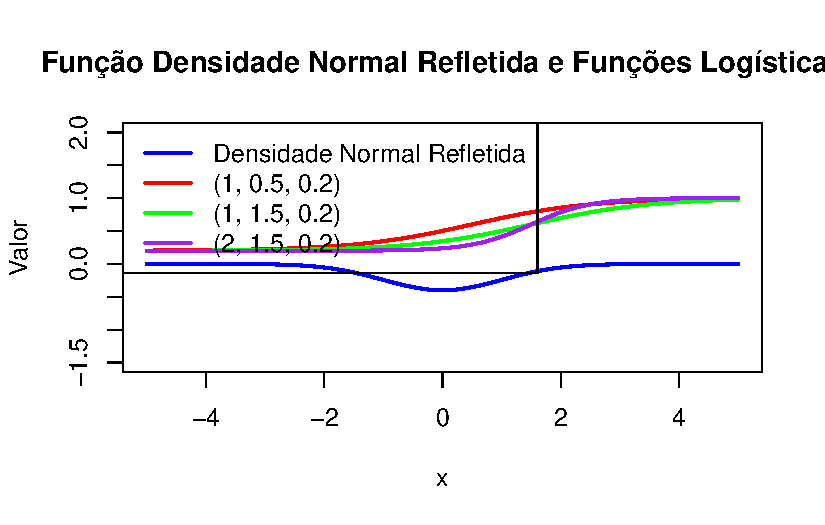
\includegraphics{intro_files/figure-pdf/unnamed-chunk-6-1.pdf}

\begin{Shaded}
\begin{Highlighting}[]
\CommentTok{\# Gerar n = 1000 valores da distribuição uniforme U(0, 1)}
\NormalTok{n }\OtherTok{\textless{}{-}} \DecValTok{1000}
\NormalTok{valores\_uniformes }\OtherTok{\textless{}{-}} \FunctionTok{runif}\NormalTok{(n)}

\CommentTok{\# Plotar o histograma}
\FunctionTok{hist}\NormalTok{(valores\_uniformes, }\AttributeTok{main =} \StringTok{"Histograma de uma variável aleatória U(0,1)"}\NormalTok{, }
     \AttributeTok{xlab =} \StringTok{"Valores"}\NormalTok{, }\AttributeTok{ylab =} \StringTok{"Frequência"}\NormalTok{, }\AttributeTok{col =} \StringTok{"lightblue"}\NormalTok{, }\AttributeTok{border =} \StringTok{"black"}\NormalTok{, }
     \AttributeTok{breaks =} \DecValTok{20}\NormalTok{)  }\CommentTok{\# Ajuste o número de intervalos (bins) com o argumento \textquotesingle{}breaks\textquotesingle{}}
\end{Highlighting}
\end{Shaded}

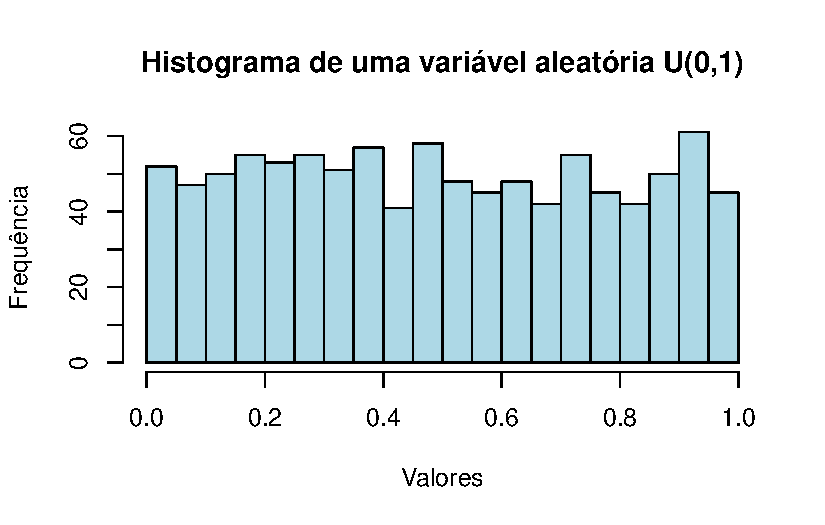
\includegraphics{intro_files/figure-pdf/unnamed-chunk-7-1.pdf}

\section{Análise Exploratória de Dados
(EDA)}\label{anuxe1lise-exploratuxf3ria-de-dados-eda}

Em estatística, a análise exploratória de dados (AED) é uma abordagem à
análise de conjuntos de dados de modo a resumir suas características
principais, frequentemente com métodos visuais. Um modelo estatístico
pode ou não ser usado, mas primariamente a AED tem como objetivo
observar o que os dados podem nos dizer além da modelagem formal ou do
processo de teste de hipóteses. Um Mini Roteiro para Realizar uma
Análise Exploratória de Dados usando a Linguagem de Programação
\(R_{4.3}\) com auxílio da IDE RStudio.

\begin{Shaded}
\begin{Highlighting}[]
\CommentTok{\# Parâmetro p para a distribuição Bernoulli}
\NormalTok{p }\OtherTok{\textless{}{-}} \FloatTok{0.3}
\NormalTok{n }\OtherTok{\textless{}{-}} \DecValTok{1000}

\CommentTok{\# Gerar n valores de uma variável aleatória Bernoulli(p)}
\NormalTok{valores\_bernoulli }\OtherTok{\textless{}{-}} \FunctionTok{rbinom}\NormalTok{(n, }\DecValTok{1}\NormalTok{, p)}

\CommentTok{\# Calcular a média e variância amostral}
\NormalTok{media\_amostral }\OtherTok{\textless{}{-}} \FunctionTok{mean}\NormalTok{(valores\_bernoulli)}
\NormalTok{variancia\_amostral }\OtherTok{\textless{}{-}} \FunctionTok{var}\NormalTok{(valores\_bernoulli)}

\CommentTok{\# Valores teóricos para média e variância}
\NormalTok{media\_teorica }\OtherTok{\textless{}{-}}\NormalTok{ p}
\NormalTok{variancia\_teorica }\OtherTok{\textless{}{-}}\NormalTok{ p }\SpecialCharTok{*}\NormalTok{ (}\DecValTok{1} \SpecialCharTok{{-}}\NormalTok{ p)}

\CommentTok{\# Exibir os resultados}
\FunctionTok{cat}\NormalTok{(}\StringTok{"Média amostral: "}\NormalTok{, media\_amostral, }\StringTok{"}\SpecialCharTok{\textbackslash{}n}\StringTok{"}\NormalTok{)}
\end{Highlighting}
\end{Shaded}

\begin{verbatim}
Média amostral:  0.288 
\end{verbatim}

\begin{Shaded}
\begin{Highlighting}[]
\FunctionTok{cat}\NormalTok{(}\StringTok{"Média teórica: "}\NormalTok{, media\_teorica, }\StringTok{"}\SpecialCharTok{\textbackslash{}n}\StringTok{"}\NormalTok{)}
\end{Highlighting}
\end{Shaded}

\begin{verbatim}
Média teórica:  0.3 
\end{verbatim}

\begin{Shaded}
\begin{Highlighting}[]
\FunctionTok{cat}\NormalTok{(}\StringTok{"Variância amostral: "}\NormalTok{, variancia\_amostral, }\StringTok{"}\SpecialCharTok{\textbackslash{}n}\StringTok{"}\NormalTok{)}
\end{Highlighting}
\end{Shaded}

\begin{verbatim}
Variância amostral:  0.2052613 
\end{verbatim}

\begin{Shaded}
\begin{Highlighting}[]
\FunctionTok{cat}\NormalTok{(}\StringTok{"Variância teórica: "}\NormalTok{, variancia\_teorica, }\StringTok{"}\SpecialCharTok{\textbackslash{}n}\StringTok{"}\NormalTok{)}
\end{Highlighting}
\end{Shaded}

\begin{verbatim}
Variância teórica:  0.21 
\end{verbatim}

A média amostral está próximo da média teórica, enquanto que a Variância
amostral também está próxima da média teórica

\begin{Shaded}
\begin{Highlighting}[]
\CommentTok{\# Parâmetro p para a distribuição Bernoulli}
\NormalTok{p }\OtherTok{\textless{}{-}} \FloatTok{0.5}
\NormalTok{n }\OtherTok{\textless{}{-}} \DecValTok{10}

\CommentTok{\# Gerar n valores de uma variável aleatória Bernoulli(p)}
\NormalTok{valores\_bernoulli }\OtherTok{\textless{}{-}} \FunctionTok{rbinom}\NormalTok{(n, }\DecValTok{1}\NormalTok{, p)}

\CommentTok{\# Calcular a média e variância amostral}
\NormalTok{media\_amostral }\OtherTok{\textless{}{-}} \FunctionTok{mean}\NormalTok{(valores\_bernoulli)}
\NormalTok{variancia\_amostral }\OtherTok{\textless{}{-}} \FunctionTok{var}\NormalTok{(valores\_bernoulli)}

\CommentTok{\# Valores teóricos para média e variância}
\NormalTok{media\_teorica }\OtherTok{\textless{}{-}}\NormalTok{ p}
\NormalTok{variancia\_teorica }\OtherTok{\textless{}{-}}\NormalTok{ p }\SpecialCharTok{*}\NormalTok{ (}\DecValTok{1} \SpecialCharTok{{-}}\NormalTok{ p)}

\CommentTok{\# Exibir os resultados}
\FunctionTok{cat}\NormalTok{(}\StringTok{"Média amostral: "}\NormalTok{, media\_amostral, }\StringTok{"}\SpecialCharTok{\textbackslash{}n}\StringTok{"}\NormalTok{)}
\end{Highlighting}
\end{Shaded}

\begin{verbatim}
Média amostral:  0.4 
\end{verbatim}

\begin{Shaded}
\begin{Highlighting}[]
\FunctionTok{cat}\NormalTok{(}\StringTok{"Média teórica: "}\NormalTok{, media\_teorica, }\StringTok{"}\SpecialCharTok{\textbackslash{}n}\StringTok{"}\NormalTok{)}
\end{Highlighting}
\end{Shaded}

\begin{verbatim}
Média teórica:  0.5 
\end{verbatim}

\begin{Shaded}
\begin{Highlighting}[]
\FunctionTok{cat}\NormalTok{(}\StringTok{"Variância amostral: "}\NormalTok{, variancia\_amostral, }\StringTok{"}\SpecialCharTok{\textbackslash{}n}\StringTok{"}\NormalTok{)}
\end{Highlighting}
\end{Shaded}

\begin{verbatim}
Variância amostral:  0.2666667 
\end{verbatim}

\begin{Shaded}
\begin{Highlighting}[]
\FunctionTok{cat}\NormalTok{(}\StringTok{"Variância teórica: "}\NormalTok{, variancia\_teorica, }\StringTok{"}\SpecialCharTok{\textbackslash{}n}\StringTok{"}\NormalTok{)}
\end{Highlighting}
\end{Shaded}

\begin{verbatim}
Variância teórica:  0.25 
\end{verbatim}

\begin{Shaded}
\begin{Highlighting}[]
\CommentTok{\# Parâmetro para a distribuição normal N(0,1)}
\NormalTok{n }\OtherTok{\textless{}{-}} \DecValTok{1000}

\CommentTok{\# Gerar n valores de uma variável aleatória normal N(0, 1)}
\NormalTok{valores\_normais }\OtherTok{\textless{}{-}} \FunctionTok{rnorm}\NormalTok{(n, }\AttributeTok{mean =} \DecValTok{0}\NormalTok{, }\AttributeTok{sd =} \DecValTok{1}\NormalTok{)}

\CommentTok{\# Calcular a média e variância amostral}
\NormalTok{media\_amostral }\OtherTok{\textless{}{-}} \FunctionTok{mean}\NormalTok{(valores\_normais)}
\NormalTok{variancia\_amostral }\OtherTok{\textless{}{-}} \FunctionTok{var}\NormalTok{(valores\_normais)}

\CommentTok{\# Valores teóricos para média e variância}
\NormalTok{media\_teorica }\OtherTok{\textless{}{-}} \DecValTok{0}
\NormalTok{variancia\_teorica }\OtherTok{\textless{}{-}} \DecValTok{1}

\CommentTok{\# Exibir os resultados}
\FunctionTok{cat}\NormalTok{(}\StringTok{"Média amostral: "}\NormalTok{, media\_amostral, }\StringTok{"}\SpecialCharTok{\textbackslash{}n}\StringTok{"}\NormalTok{)}
\end{Highlighting}
\end{Shaded}

\begin{verbatim}
Média amostral:  -0.02016776 
\end{verbatim}

\begin{Shaded}
\begin{Highlighting}[]
\FunctionTok{cat}\NormalTok{(}\StringTok{"Média teórica: "}\NormalTok{, media\_teorica, }\StringTok{"}\SpecialCharTok{\textbackslash{}n}\StringTok{"}\NormalTok{)}
\end{Highlighting}
\end{Shaded}

\begin{verbatim}
Média teórica:  0 
\end{verbatim}

\begin{Shaded}
\begin{Highlighting}[]
\FunctionTok{cat}\NormalTok{(}\StringTok{"Variância amostral: "}\NormalTok{, variancia\_amostral, }\StringTok{"}\SpecialCharTok{\textbackslash{}n}\StringTok{"}\NormalTok{)}
\end{Highlighting}
\end{Shaded}

\begin{verbatim}
Variância amostral:  0.9588775 
\end{verbatim}

\begin{Shaded}
\begin{Highlighting}[]
\FunctionTok{cat}\NormalTok{(}\StringTok{"Variância teórica: "}\NormalTok{, variancia\_teorica, }\StringTok{"}\SpecialCharTok{\textbackslash{}n}\StringTok{"}\NormalTok{)}
\end{Highlighting}
\end{Shaded}

\begin{verbatim}
Variância teórica:  1 
\end{verbatim}

\bookmarksetup{startatroot}

\chapter*{References}\label{references}
\addcontentsline{toc}{chapter}{References}

\markboth{References}{References}

\begin{enumerate}
\def\labelenumi{\arabic{enumi}.}
\item
  H. Wickham. ggplot2: Elegant Graphics for Data Analysis.
  Springer-Verlag New York, 2016.
\item
  Wickham H, François R, Henry L, Müller K, Vaughan D (2023).
  \emph{dplyr: A Grammar of Data Manipulation}. R package version 1.1.4,
  \url{https://CRAN.R-project.org/package=dplyr}.
\item
  Xie Y, Cheng J, Tan X (2024). \emph{DT: A Wrapper of the JavaScript
  Library `DataTables'}. R package version 0.33,
  \url{https://CRAN.R-project.org/package=DT}.
\end{enumerate}



\end{document}
